\documentclass[10pt]{article}
\usepackage[polish]{babel}
\usepackage[utf8]{inputenc}
\usepackage[T1]{fontenc}
\usepackage{amsmath}
\usepackage{amsfonts}
\usepackage{amssymb}
\usepackage[version=4]{mhchem}
\usepackage{stmaryrd}
\usepackage{graphicx}
\usepackage[export]{adjustbox}
\graphicspath{ {./images/} }

\title{KLASY PIERWSZE I DRUGIE }

\author{}
\date{}


\begin{document}
\maketitle
\begin{enumerate}
  \item Oblicz różnicę:
\end{enumerate}

\[
\left(1^{2}+2^{2}+3^{2}+\cdots+2023^{2}\right)-(1 \cdot 3+2 \cdot 4+3 \cdot 5+\cdots+2022 \cdot 2024)
\]

\begin{enumerate}
  \setcounter{enumi}{1}
  \item Ile liczb trzycyfrowych podzielnych przez 9 ma następującą własność: suma cyfr ilorazu tej liczby przez 9 jest o 9 mniejsza od sumy jej cyfr?
  \item Rysunek obok przedstawia kwadratową płytkę. Narysowane na niej linie krzywe są ćcwiartkami okręgów o promieniu równym połowie boku płytki. Długość takiej ćwiartki okręgu jest równa 5 dm. Z 16 takich płytek budujemy kwadrat. Jaką maksymalną długość może mieć nieprzerwana linia utworzona z tych ćwiartek okręgów?\\
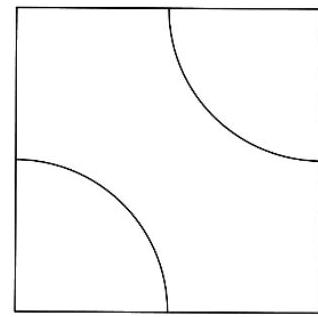
\includegraphics[max width=\textwidth, center]{2024_11_21_982dd79c5ffd7d726118g-1}
\end{enumerate}

\section*{KLASY TRZECIE I CZWARTE}
\begin{enumerate}
  \item W szkolnym turnieju piłki ręcznej każda drużyna rozegrała z każdą inną dokładnie jeden mecz. Drużyna zwycięska zdobywała 2 punkty, przegrana 0 punktów, w przypadku zaś remisu obie drużyny otrzymywały po jednym punkcie. Zwycięzca turnieju zdobył w czasie całych rozgrywek 7 punktów, drużyna druga 5 punktów, a drużyna trzecia 3 punkty. Ile punktów zdobyła drużyna, która zajęła ostatnie miejsce?
  \item Funkcja \(f\) określona jest na zbiorze liczb naturalnych wzorem
\end{enumerate}

\[
f(n)=\left\{\begin{array}{cc}
n+5 & \text { gdy } n \text { jest liczbą nieparzystą } \\
\frac{n}{2} & \text { gdy } n \text { jest liczbą parzystą }
\end{array}\right.
\]

Ile jest równa suma cyfr liczby nieparzystej \(k\), dla której \(f(f(f(k)))=35\) ?\\
3. Ile co najwyżej trójelementowych podzbiorów można utworzyć z elementów zbioru siedmioelementowego w taki sposób, aby każde dwa z powstałych podzbiorów miały dokładnie jeden element wspólny?


\end{document}